\chapter{Material und Methoden}
\label{cha:config}

Dieses Kapitel gibt einen Überblick der im Projekt verwendeten Hardware und Software.


\section{Plattformen}

Als Minicomputer bestehend aus einer einzelnen Platine wurden Raspberry Pi und Arduino entwickelt um Nutzer an digitale Technik heranzuführen und dabei spielerisch Programmierfähigkeiten zu vermitteln. Die Fülle an Schnittstellen macht die Plattform ideal für das Prototyping interaktiver Anwendungen unter Verwendung von Sensorik und Aktorik. 

\subsection{Raspberry Pi}

Der Raspberry Pi ist die vorrangige Entwicklungsplattform des Projekts. Das Institut für Telematik stellt zwei Versionen zur Verfügung, Diese unterscheiden sich in Ausstattung und Leistungsfähigkeit und sind in Bild \ref{img:rpi} dargestellt. Die Platinen bieten einen HDMI zur direkten Bildschirmausgabe und werden mit dem Betriebssystem Raspbian betrieben, welches auf Debian basiert. Konzipiert für die ARM-Prozessoren und vergleichsweise geringen Ressourcen der Raspberries bietet das System mehr als 35.000 auf Performance ausgelegt Softwarepakete. Die im Projekt verwendete Version Raspbian Jessie Lite verfügt über keine grafische Benutzeroberfläche und ist nur knapp $1,5GB$ groß. Das Besondere an der Platine sind die General Purpose Input Output Ports (GPIO), welche wahlweise als Eingang oder Ausgang konfiguriert werden können. Der verbaute BCM2835 Mikrocontroller gibt der Nummerierung der Pins den offiziellen Namen BCM-Numbering. In Bild \ref{img:RPi_GPIO} ist das BCM-Numbering auf dem T-Cobler dargestellt. Dieser verbindet die Platine mit dem verwendeten Breadboard.

\begin{figure}
	\centering
	\subfigure[Raspberry Pi 2 B - 4x 900 MHz, 1GB RAM, externes WLAN]{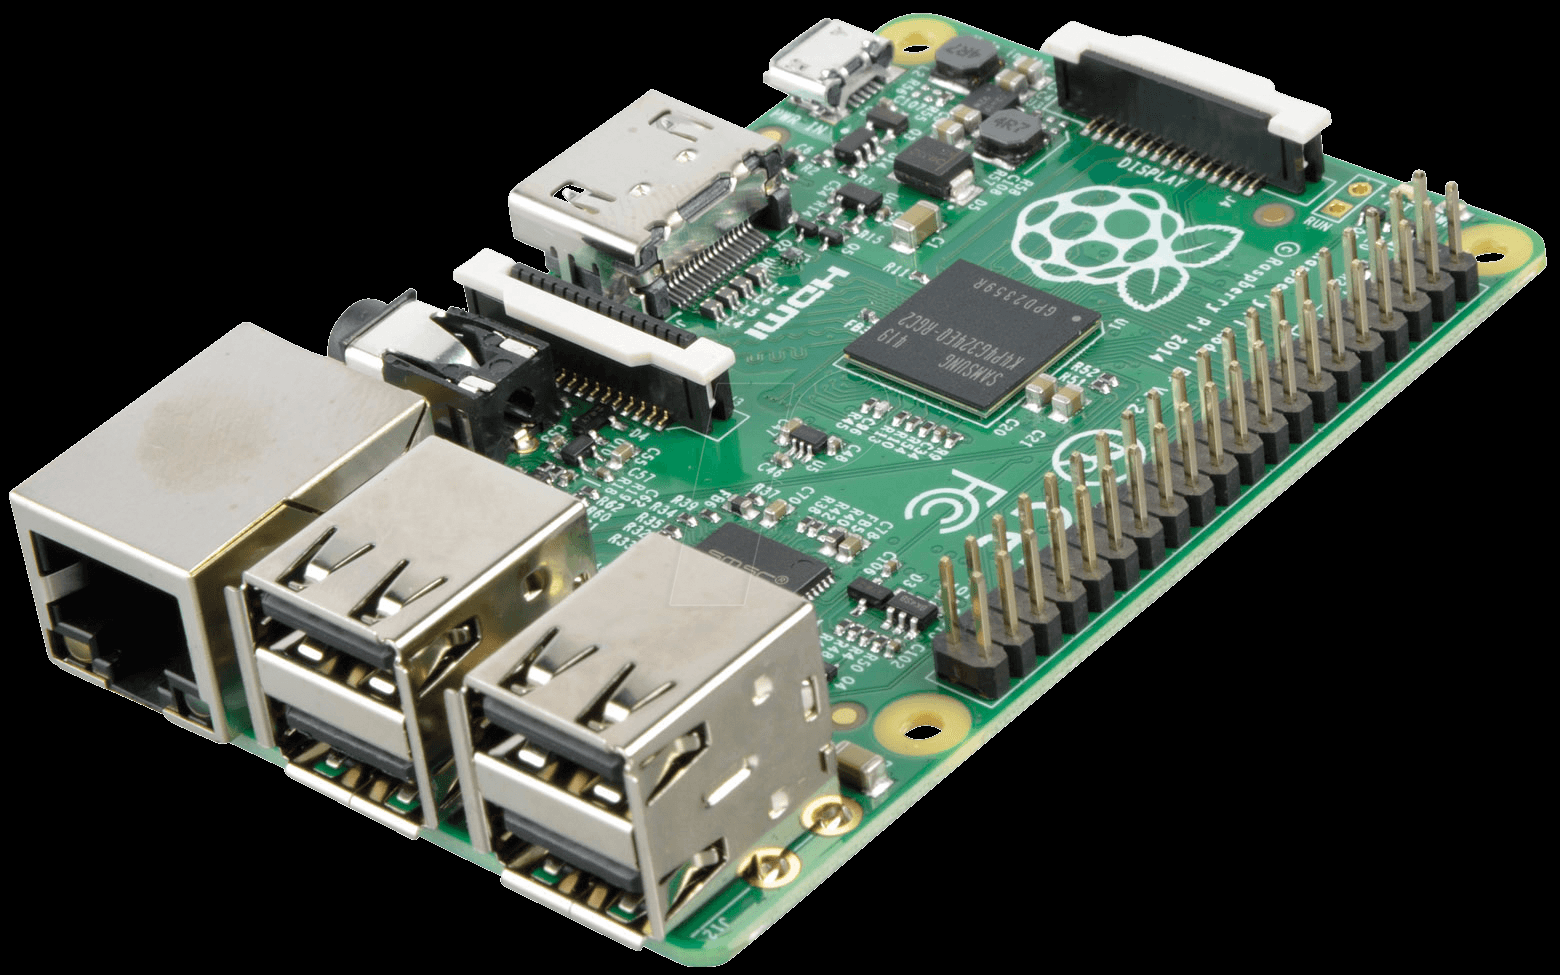
\includegraphics[width=0.45\textwidth]{figures/RPi2.png}}
	\label{img:rpi2b}
	\subfigure[Raspberry Pi 3 B - 4x 1,2 GHz, 1GB RAM, integriertes WLAN und
Bluetooth]{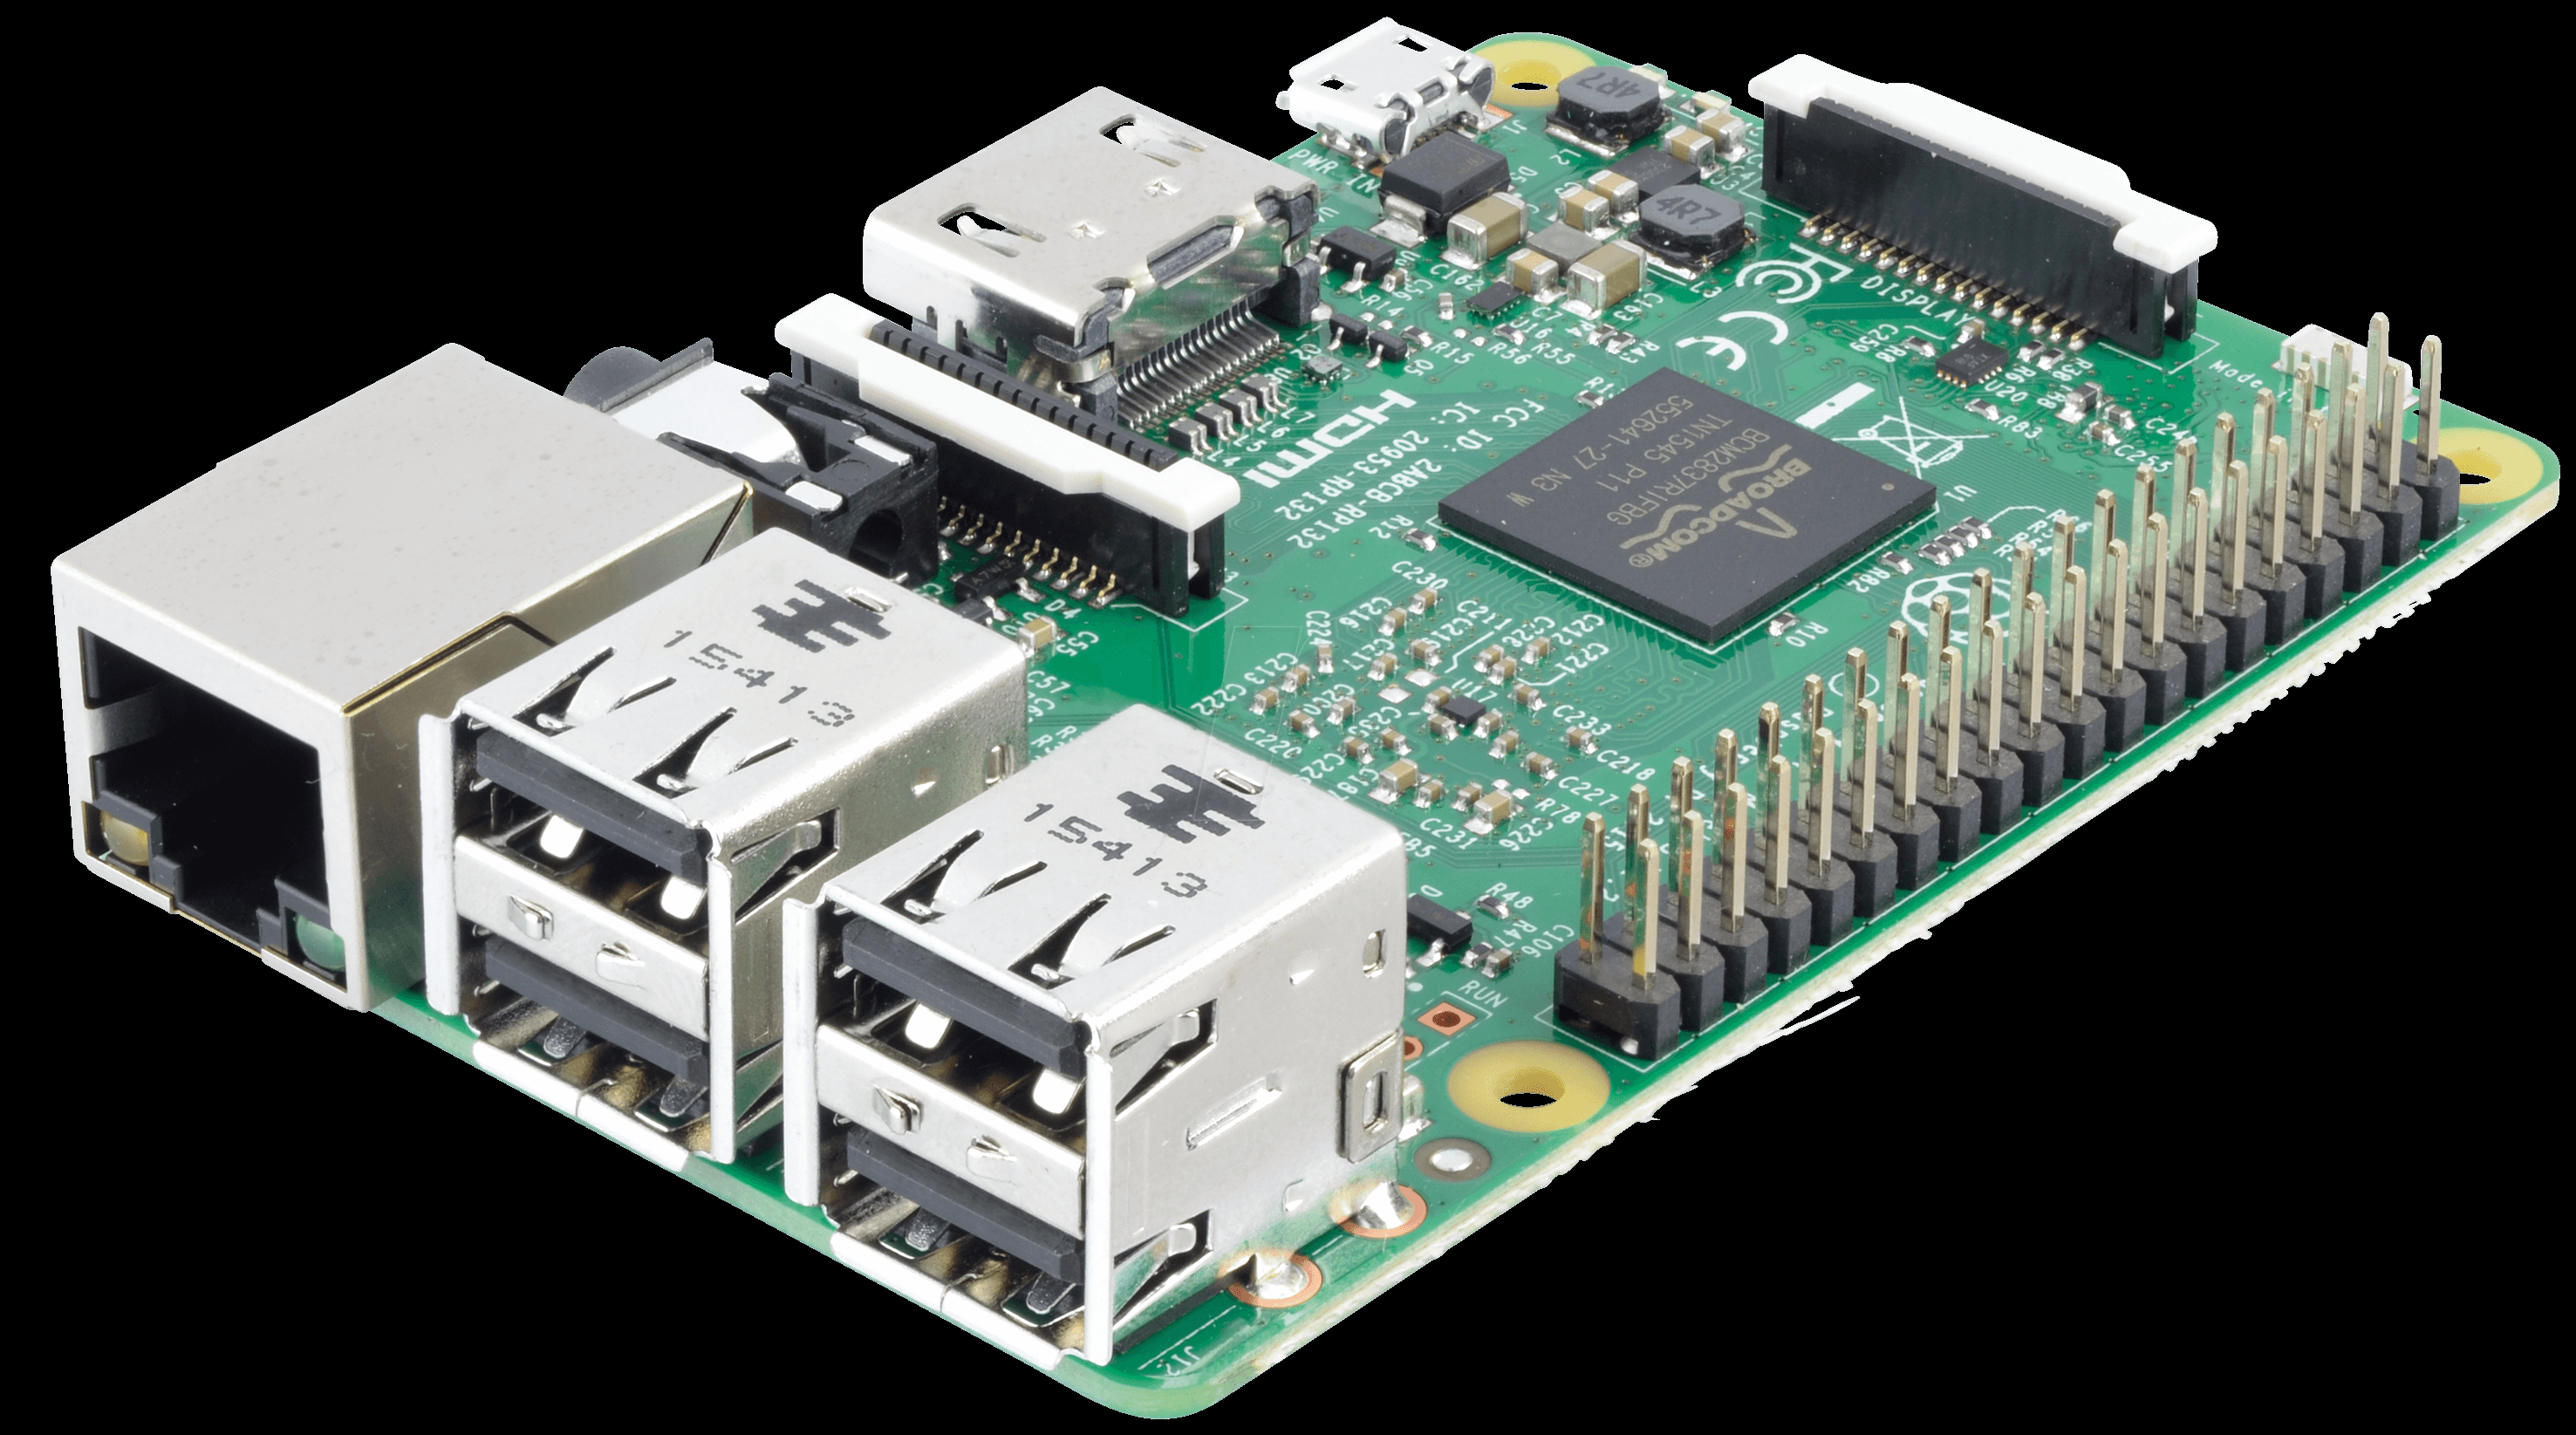
\includegraphics[width=0.45\textwidth]{figures/RPi3.png}}
	\label{img:rpi3b}
	\caption{Versionen der durch das Institut für Telematik bereitgestellten Raspberry Pi}
	\addloflink{https://www.arduino.cc/en/Main/arduinoBoardUno}
	\label{img:rpi}
\end{figure}

\begin{figure}
	\centering
	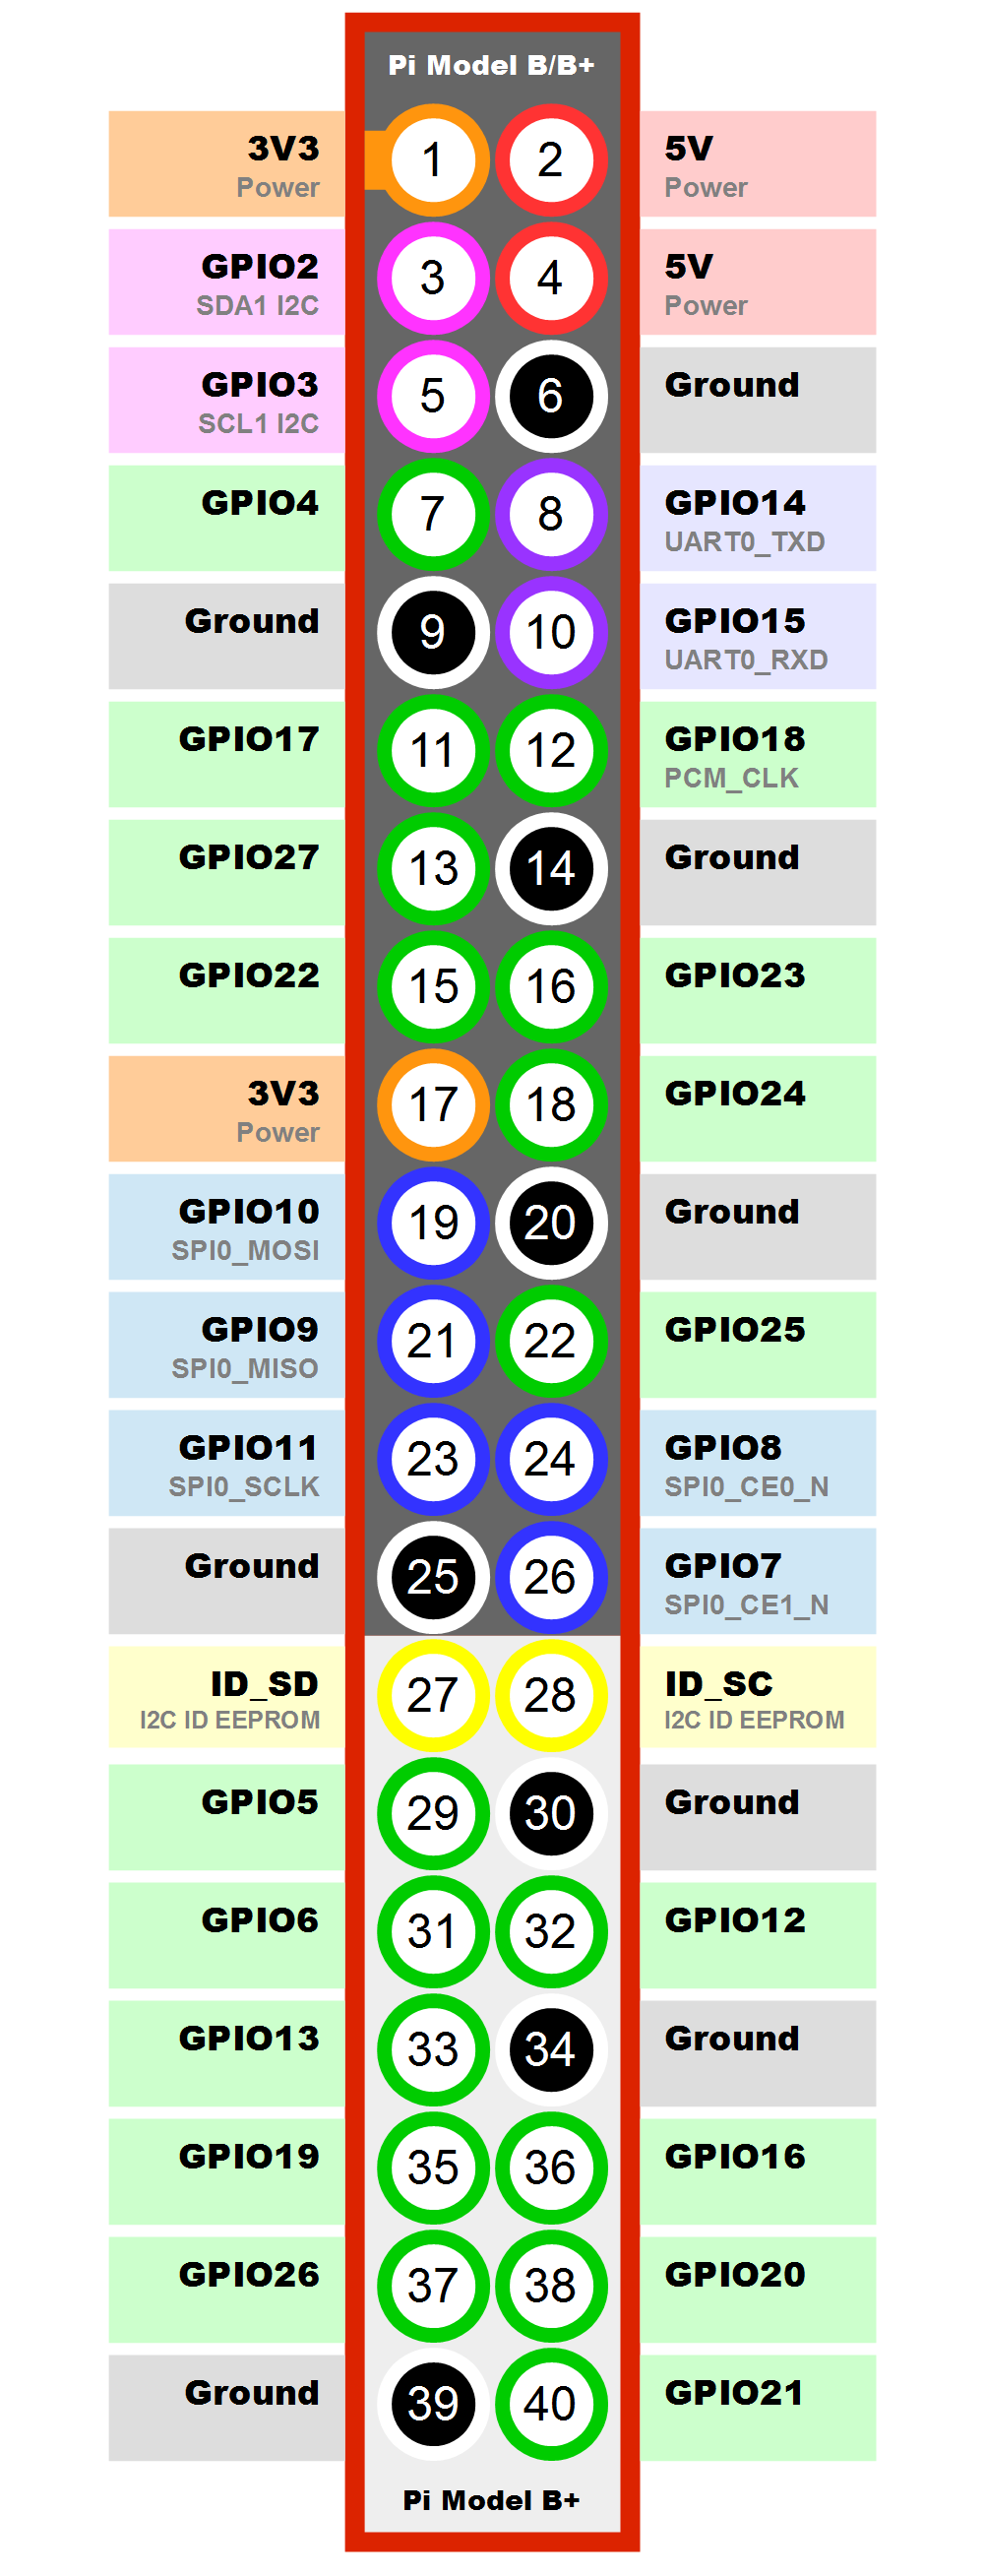
\includegraphics[width=0.5\textwidth]{figures/RPi_GPIO.png}
	\caption{BCM-Numbering der GPIO Ports am Raspberry Pi}
	\addloflink{www.raspberrypi-spy.co.uk}
	\label{img:RPi_GPIO}
\end{figure}


\subsection{Arduino}

Der Arduino Uno basiert auf dem ATmega328P Microcontroller und bietet neben 14 digitalen I/O-Pins auch sechs analoge Pins. Diese sind an mit einem 6Kanal A/D-Wandler verbunden wodurch u.A. das Auslesen analoger Sensorik ermöglicht wird. Das Board kommt mit seiner eigenen Entwicklungsumgebeung, der Arduino IDE, diese wird in C programmiert und bietet umfangreiche Bibliotheken zum Ansteuern der einzelnen Funktionalitäten. Das Layout der Platine ist in Bild \ref{img:arduino_layout} dargestellt.


\begin{figure}
	\centering
	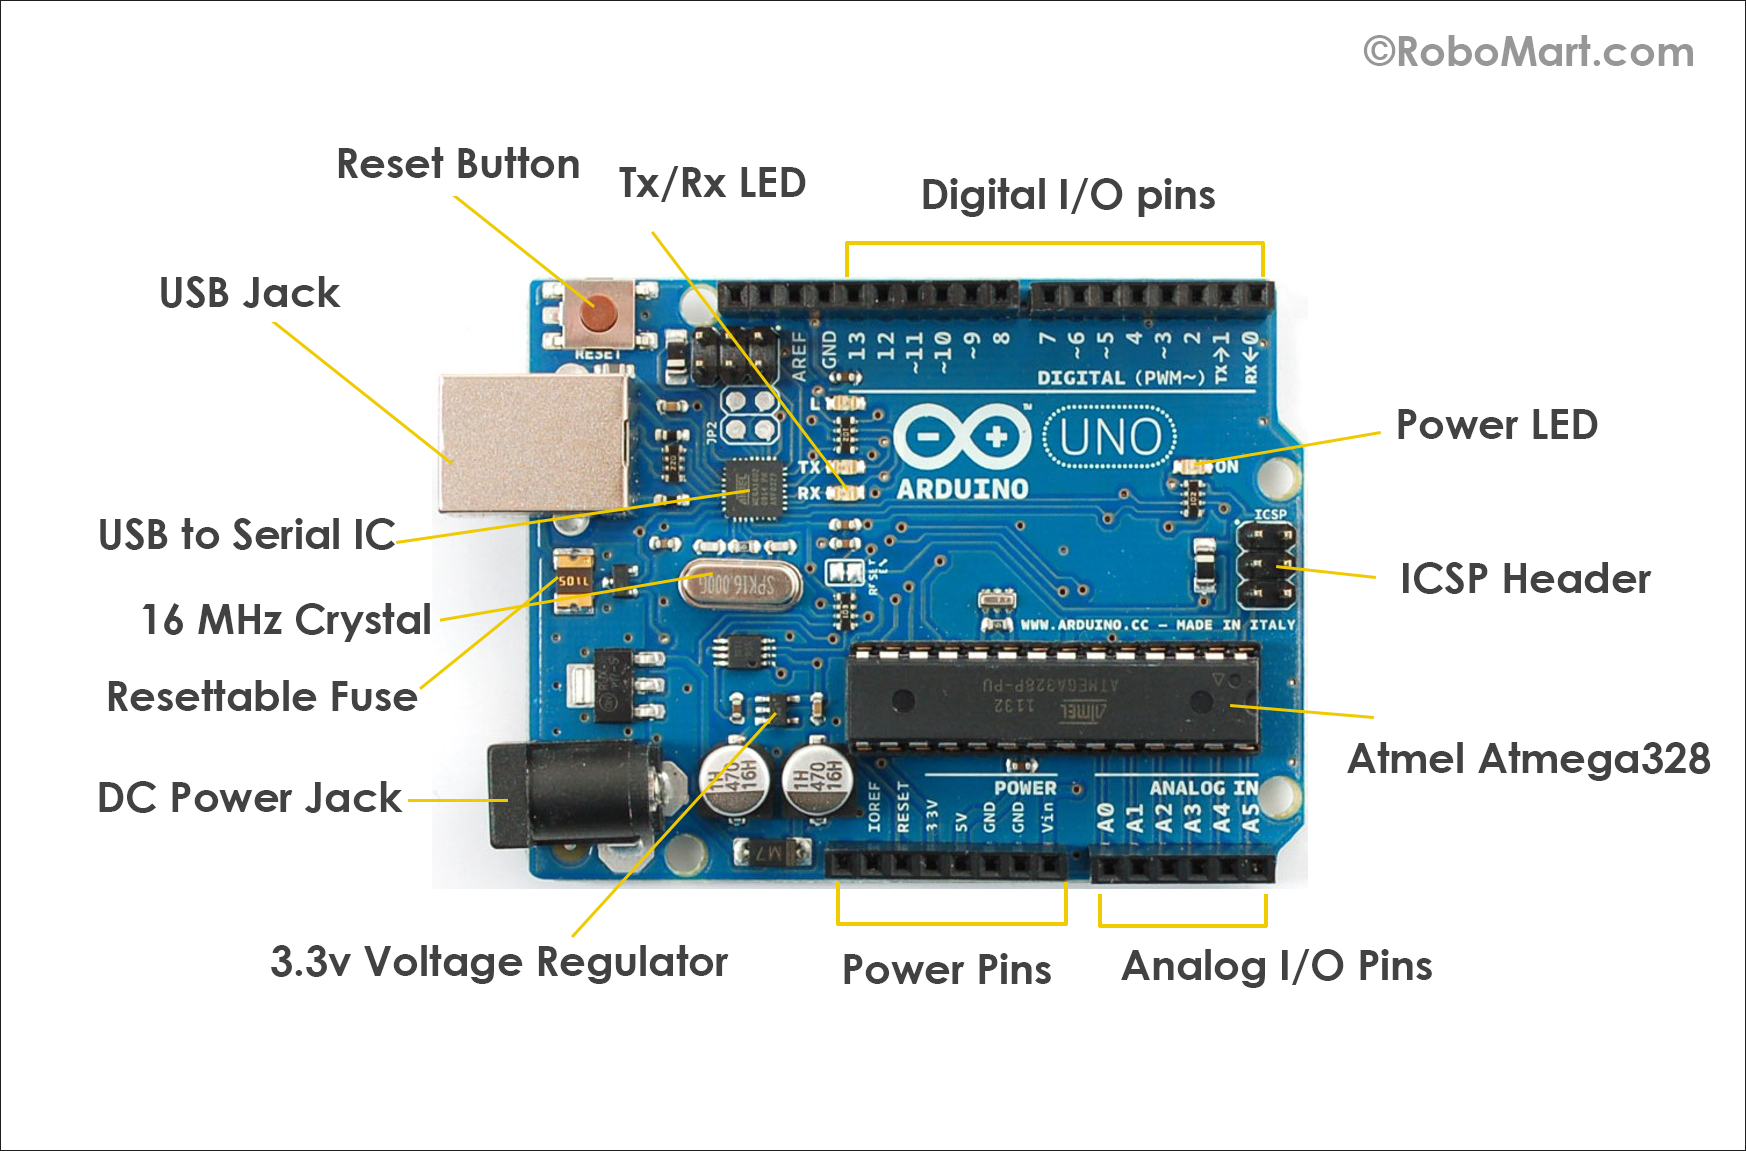
\includegraphics[width=0.5\textwidth]{figures/arduino_layout.png}
	\caption{Layout Arduino Uno}
	\addloflink{www.robomart.com/blog/wp-content/uploads/2015/07/Arduino_Components_layout-1024x675.png}
	\label{img:arduino_layout}
\end{figure}


\section{Software}

\begin{list}{}{}
 \item \textbf{Arduino IDE} Für die Programmierung des Arduino bereitgestellt Entwicklungsumgeben. Wird in C programmiert und stellt eine umfangreiche Bibliothek zum einfachen Ansteuern der Platine bereit.
 \item \textbf{PI4J} Bibliothek zum Ansteuern der Input/Output-Ports des Raspberry Pi in Java.
 \item \textbf{RXTX} Bibliothek für die Nutzung der seriellen Schnittstelle des Pi in Java.
 \item \textbf{Maven} Java basiertes Build-Management Tool. Ermöglicht die standardisierte Erzeugung von Paketen.
 \item \textbf{Git} Ein Open Source Programm zur Versionsverwaltung von Dateien. Verwaltet die Versionierung von gemeinsam genutzten Dateien und ermöglicht damit ein koordiniertes Arbeiten an Projekten mit mehreren Entwicklern.
 \item \textbf{Eclipse} Integrierte Entwicklungsumgebung u.a. für Java mit der Möglichkeit eine Vielzahl von Plugins zur Optimierung des Entwicklungsprozesses einzubinden.
\end{list}

\subsection{Semantic Web}

Der Kontext bestimmt die Beziehung zwischen miteinander verbunden Objekten oder Informationen und impliziert zusätzliche Informationen, welche nicht durch die unabhängige Betrachtung der einzelnen Komponenten ersichtlich sind. Während Menschen in der Lage sind den Kontext zu erfassen, daraus intuitiv Verknüpfungen zu bilden und auf weitere Informationen zu schließen, muss dieses Wissen für Maschinen explizit bereitgestellt werden. Das Semantic Web ist die technische Umsetzung dieses Umstandes und zielt darauf ab Datenaustausch und Auswertung durch Computer zu vereinfachen. Unter der Führung des W3C wird seit 2004 die standardisierte Web Ontology Language (OWL) entwickelt um Ontologien in einer formalen Beschreibungssprache konzipieren, veröffentlichen und teilen zu können. Damit können die Eigenschaften einer Domäne in maschinenverständlicher Form beschrieben werden.

\subsection{SSP}

Der Smart Service Proxy wurde durch Oliver Kleine am ITM der Universität zu Lübeck entwickelt und implementiert um nach dem Konzept des Semantic Web ein digitales Abbild der Gegenwart zu ermöglichen. Dazu können Sensorik und Aktorik am SSP registriert und deren Status kontinuierlich aktualisert werden. Clients können den Zustand aller registrierten, beobachtbaren Ressourcen am SSP abrufen und für ihre Zwecke nutzen. Damit bildet der SSP die Grundlage für die Integration digitaler Services in eine natürliche Umgebung.  

\subsection{nCOAP}
\label{subsec:ncoap}

Das Constraint Application Protocol ist eine leichtgewichtige Alternative zu HTTP die den Zugriff auf Ressourcen in ressourcen-beschränkten Umgebungen realisiert. Statt TCP wird UDP genutzt um asynchronen Datenaustausch zu ermöglichen. Im Vergleich zu HTTP reduzieren die komprimierten binären Header und Body Abschnitte den Overhead der Kommunikation. Die Gemeinsamkeiten zu HTTP, wie Anfragemethoden $GET$, $PUT$, $POST$ und $DELETE$ oder ähnliche Fehlercodes ermöglichen die einfache Implementierung von Cross-Protocol-Proxies. Jede Coap Nachricht ist aufgebaut aus einem 4Byte Header, den CoAP-Optionen und dem CoAP-Body, welcher die Payload enthält. Der Aufbau einer Coap-Nachricht wird in Bild \ref{img:coap_msg} dargestellt. In diesem Projekt wird die durch Oliver Kleine entwickelte Java Implementierung nCoAP verwendet um mit dem Smart Service Proxy (SSP) zu kommunizieren. 

\begin{figure}
	\centering
	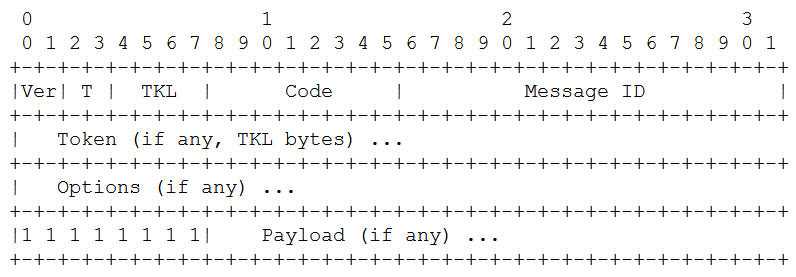
\includegraphics[width=0.85\textwidth]{figures/coap_msg.png}
	\caption{Coap Nachrichtenformat}
	\addloflink{https://tools.ietf.org/html/rfc7252}
	\label{img:coap_msg}
\end{figure}


\subsection{Informationsdienste}
\label{subsec:webinfo}

\subsubsection{iCal}
\label{subsubsec:ical}

Das Datenformat iCalendar definiert den Internet Media Type \textit{text/calendar} in der RFC 5545. Es wurde durch die Arbeitsgruppe Calsify der der Internet Engineering Task Force entwickelt um die Veröffentlichung von Terminen und die gemeinsame Nutzung von Kalendern zu ermöglichen. Das Datenformat selbst ist nicht auf  ein spezifisches Netzwerkprotokoll beschränkt. Daher ist in der RFC 5546 das Transport Independent Interoperability Protocol (iTIP) beschrieben, welches den plattformübergreifenden Austausch realisiert. 

\subsubsection{Weather API}
\label{subsubsec:weather}

Der Servicedienstleister \url{openweathermap.org} bietet neben Anderen die Möglichkeit Datensätze zum aktuellen und prognostizierten Wetter nahezu aller Regionen der Erde abzurufen. So kann beispielsweise mit der Anfrage \url{api.openweathermap.org/data/2.5/weather?q=London,uk} die momentan Wetterlage in London in Form einer \textit{*.json} abgerufen werden. In der Regel ist die Anzahl der möglichen Anfragen pro Stunde für das kostenlose Abgebot begrenzt. Auch weiterführende Funktionen wie 16-Tage Vorhersagen oder detailierte Wetterkarten sind Premiumkunden vorbehalten.

\subsubsection{RSS}
\label{subsubsec:rss}

Das \textit{Rich Site Summary} ist ein standardisiertes Format für die Zusammenfassung von Informationen und Aktualisierungen auf Webseiten. Daher auch die alternative Bezeichnung \textit{Really Simple Syndication}. Dabei wird ein News-Feed durch eine \textit{URI} identifiziert und durch Attribute wie Titel, Veröffentlichungsdatum oder Sprache beschrieben. Dem Feed zugeordnet sind wiederrum Feed-Nachrichten, welche die eigentlichen Informationen in vergleichbaren Attributen enthalten. Diese hierarchische Struktur wird in der Auszeichnungssprache XML beschrieben.

\subsection{OpenCV}
\label{subsec:opencv}

- Bibliothek für Echtzeit Computer Vision



\section{Bauteile}
\label{cha:components}

Dieser Abschnitt stellt die im Projekt verwendeten Bauteile vor und gibt einen kurzen Überblick über Eigenschaften und Funktionsweise. Mit fortschreitendem Projektverlauf wird die Sektion stetig erweitert werden. 

\subsection{Leuchtdiode}

Die Leuchtdiode ist ein Halbleiterbauelement, welches im Aufbau einer pn-Halbleiterdiode entspricht und sich mit diesen die gleichen Grundeigenschaften teilt. In Durchflussrichtung schließt sie einen Stromkreis, während sie entgegen der Durchflussrichtung sperrt. Im Betrieb strahlt der verbaute Halbleiterkristall Licht ab dessen Wellenlänge von der Dotierung und Art des verwendeten Materials abhängt. So können Leuchtdioden im sichtbaren Bereich Licht in verschieden Farben erzeugen, aber auch infrarote oder ultraviolette Strahlung abgeben. Die LED wird z.B. in Produkten wie Taschenlampen, Flachbildschirmen oder als Signalgeber in Sensoren eingesetzt.

Die Eigenschaften von Leuchtdioden sind abhängig von der jeweiligen Art, so unterscheiden sich die Spezifikationen für alle verfügbaren Modelle. Um eine Überlastung zu vermeiden und die Lebensdauer der Bauteile zu vermeiden sollten Leuchtdioden nur mit einem Vorwiderstand betrieben werden. Dieser muss auf die gegebene Spannungsquelle und das verwendete Bauteil abgestimmt werden.

\begin{table}[]
\centering
\caption{LED Flussspannungen}
\label{my-label}
\begin{tabular}{@{}|l|l|@{}}
\toprule
\rowcolor[HTML]{BBDAFF} 
Art          & Flussspannung \\ \midrule
Infrarot     & 1,2 - 1,8V    \\ \midrule
\rowcolor[HTML]{BBDAFF} 
Rot          & 1,6 - 2,2V    \\ \midrule
Gelb, Grün   & 1,9 - 2,5V    \\ \midrule
\rowcolor[HTML]{BBDAFF} 
Blau, Weiß   & 2,7 - 3,5V    \\ \midrule
Ultraviolett & 3,1 -4,5V     \\ \bottomrule
\end{tabular}
\end{table}

\subsection{Fotowiderstand}

Der Fotowiderstand ist ein lichtempfindliches Halbleiterbauelement dessen ohmscher Widerstand von der Stärke des einfallenden Lichts abhängig ist. In elektrischen Schaltungen wird das Bauteil Signalaufnehmer zur Erfassung des Umgebungslichts verwendet. Beispielhafte Anwendungen sind Dämmerungsschalter oder Belichtungsmesser von Kameras. In Reihe mit einem korrekt dimensionierten Widerstand entsteht ein Spannungsteiler über den der Widerstand gemessen werden kann.




%%%%% Emacs-related stuff
%%% Local Variables: 
%%% mode: latex
%%% TeX-master: "../../main"
%%% End: 
